\begin{center}
    \textbf{Geração 80}
\end{center}

\begin{figure}[h]
    \centering
    \label{fig:geracao01}
    
    \begin{tabular}{rl}
        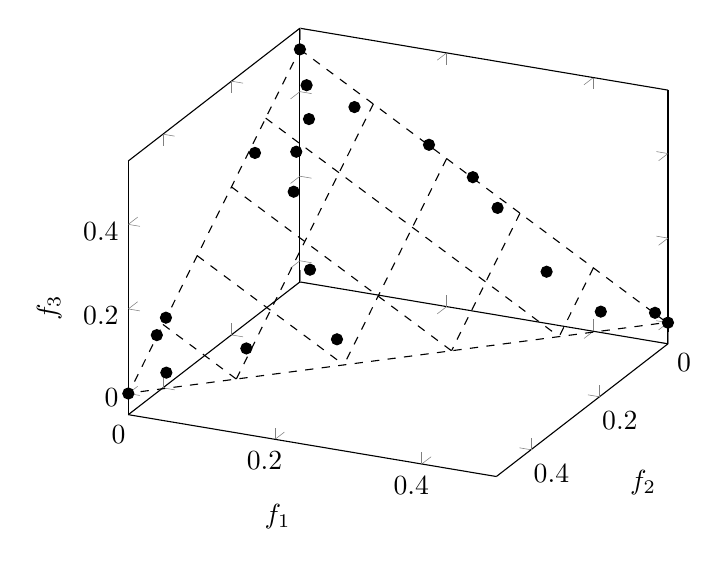
\begin{tikzpicture}[scale=1.0]
        	\begin{axis}[xlabel=$f_2$, ylabel=$f_1$, zlabel=$f_3$, view/h=115]
        		
    			\addplot3[style={dashed}]coordinates {
    			    (0., 0., 0.5) (0., 0.5, 0.) (0.5, 0., 0.) (0., 0., 0.5)
    			};
    			
    			\addplot3[style={dashed}]coordinates {(0., 0.1, 0.4) (0.4, 0.1, 0.)};
    			\addplot3[style={dashed}]coordinates {(0., 0.2, 0.3) (0.3, 0.2, 0.)};
    			\addplot3[style={dashed}]coordinates {(0., 0.3, 0.2) (0.2, 0.3, 0.)};
    			\addplot3[style={dashed}]coordinates {(0., 0.4, 0.1) (0.1, 0.4, 0.)};
    			
    			\addplot3[style={dashed}]coordinates {(0.4, 0., 0.1) (0.4, 0.1, 0.)};
    			\addplot3[style={dashed}]coordinates {(0.3, 0., 0.2) (0.3, 0.2, 0.)};
    			\addplot3[style={dashed}]coordinates {(0.2, 0., 0.3) (0.2, 0.3, 0.)};
    			\addplot3[style={dashed}]coordinates {(0.1, 0., 0.4) (0.1, 0.4, 0.)};
    			
    			\addplot3[only marks] coordinates {
            		(0.501151, 0.000000, 0.000000) (0.000000, 0.501703, 0.000000) (0.000000, 0.000000, 0.500000) (0.041065, 0.355436, 0.103501) (0.000000, 0.235731, 0.266484) (0.156883, 0.064729, 0.280477) (0.359699, 0.094880, 0.045671) (0.013573, 0.275784, 0.214028) (0.000000, 0.175953, 0.325635) (0.040601, 0.429121, 0.030327) (0.066853, 0.043557, 0.389739) (0.279764, 0.181108, 0.042364) (0.449474, 0.027700, 0.025058) (0.112049, 0.047329, 0.341871) (0.145954, 0.006854, 0.348487) (0.018172, 0.082838, 0.399070) (0.226296, 0.119396, 0.155472) (0.417883, 0.000000, 0.085942) (0.391287, 0.000000, 0.110476) (0.035204, 0.025521, 0.444716) (0.000000, 0.484058, 0.018173) 

        		};
        	\end{axis}
	    \end{tikzpicture}
	    &
	    \begin{tikzpicture}[scale=1.0]
        	\begin{axis}[xlabel=$f_2$, ylabel=$f_1$, zlabel=$f_3$, view={45}{0}]
        		
    			\addplot3[style={dashed}]coordinates {
    			    (0., 0., 0.5) (0., 0.5, 0.) (0.5, 0., 0.) (0., 0., 0.5)
    			};
    			
    			\addplot3[only marks] coordinates {
            		(25.557095,0.000000,0.000000)(0.000000,19.177327,0.000000)(0.000000,0.000000,15.470869)(3.037656,6.672029,8.936816)(15.434954,1.229393,10.661216)(5.637196,3.829305,12.926649)(4.844314,10.655167,7.300313)(0.000000,12.296822,5.636917)(5.882303,14.099157,1.845874)(8.940586,8.204036,2.127804)(1.165727,16.318428,2.120988)(17.011234,2.938357,0.984301)(11.845078,11.870279,0.000000)(8.867463,13.563037,3.473916)(8.149641,17.784455,0.449559)(23.541033,1.906498,0.000000)(10.861441,1.290302,7.988342)(19.352375,1.159940,3.186702)(9.307486,0.776347,14.370748)(1.583821,18.413031,0.418250)(21.011899,1.370938,1.268155) 

        		};
        	\end{axis}
	    \end{tikzpicture}
	\end{tabular}
    
\end{figure}

